% ======================================================================
\subsection{Motivation}

% ----------------------------------------------------------------------
\begin{frame}
  \frametitle{Inertial manifold
    \footfullcite{Foias1988a}$^,$
    \footfullcite{Robinson1995}
  }

  An \htr{inertial manifold} is a \htb{positively invariant} and
  \htb{exponentially attracting} manifold in the \statesp.

  \vfill

  \htgc{
    Why do we care about inertial manifolds?
  }

  \pause
  \vfill

  Because it captures the asymptotic dynamics and it is \htr{finite\dmn.}

  \vfill

  Its dimension is likely much smaller than the
  number of degrees of freedom used in simulations (in principle infinite:)

\end{frame}

% ----------------------------------------------------------------------
\begin{frame}
  \frametitle{General setup\footfullcite{DasBuch}}

  Given autonomous flow $\dot{\ssp} = \vel(\ssp) \,, \quad \ssp(x, t) \in \reals^n$.

  \htb{Tangent dynamics:}
  \begin{equation}
    \label{eq:stab}
    \frac{d}{dt}\delta \ssp = A \delta\ssp \,, \quad
    A = \frac{\partial \vel}{\partial \ssp}
    \,.
  \end{equation}

  \htb{Jacobian matrix:}
  \begin{equation}
    \label{eq:jacob}
    \delta \ssp(\ssp, t)=\jMps^\zeit(\ssp_0, 0)\,\delta \ssp(\ssp_0, 0)
  \end{equation}
  \begin{equation}
    \label{eq:tangentDynamics}
    \frac{d}{dt}\jMps = A \jMps \,, \quad
    J_0 = I
    \,.
  \end{equation}

  \pause

  \htb{\Fv s:}
  \begin{equation}
    \label{eq:fm}
    \jMps_p=\jMps^{\period{p}}(\ssp, \zeit)
  \end{equation}
  \begin{equation}
    \label{eq:fv}
    \jMps_p\,\jEigvec[j]=\ExpaEig_{j}\jEigvec[j]
  \end{equation}
  \[
    \ExpaEig_{j} = \exp(\period{p}\Lyap^{(j)}_p)\
    = \exp(\period{p}\eigRe[j] + i\theta_j)
    \,.
  \]

\end{frame}

% ----------------------------------------------------------------------
\begin{frame}
  \frametitle{Covariant (Lyapunov) vectors
    \footfullcite{WoSa07}$^,$
    \footfullcite{GiChLiPo12}$^,$
    \footfullcite{KuPa12}}

  Oseledec matrices\rf{lyaos, ruelle79}:
  \begin{equation}
    \Xi^{\pm}(\ssp) :=\lim_{t\to\pm\infty}[J^t(\ssp)^\top J^{t}(\ssp)]^{1/2t}
    \label{eq:oseledets}
  \end{equation}

  {\centering
    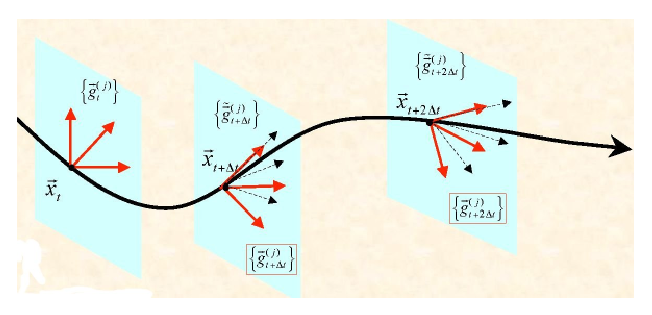
\includegraphics[width=0.7\textwidth]{GinelliFrames}
  \par}

\end{frame}

% ----------------------------------------------------------------------
\begin{frame}
  \frametitle{Decoupled tangent space
    \footfullcite{ginelli-2007-99}$^,$
    \footfullcite{YaTaGiChRa08}$^,$
    \footfullcite{TaGiCh11}
  }

  {\centering
    \includegraphics[width=0.8\textwidth]{kaza2011} %\hfill
    \scriptsize
    (from Ref.~\rf{TaGiCh11})
    \par}

\end{frame}

% ----------------------------------------------------------------------
\begin{frame}[shrink]%[allowframebreaks]
  \frametitle{\Fv s}

  \begin{center}
    \large How about using \Fv s of periodic orbits ?
  \end{center}

  \pause

  \begin{center}
    \large How to get \Fv s?
  \end{center}

  \pause

  \htb{Chain rule :}
  \begin{align*}
    \jMps^{\zeit-\zeit_{0}}(\ssp(\zeit_{0}) ,\zeit_{0})
    =
    \jMps^{\zeit-\zeit_{1}} & (\ssp(\zeit_{1}),\zeit_{1})
    \jMps^{\zeit_{1}-\zeit_{0}}(\ssp(\zeit_{0}),\zeit_{0})
    \\
    & \Downarrow \\
    \ps{\jMps}{0}=\jMps_{m}\jMps_{m-1}\cdots \jMps_{1}\,,\quad
    & \jMps_{i}\in \mathbb{R}^{n\!\times\! n},\; i\!=\!1,2,\cdots,m
    \,.
  \end{align*}


  \vfill


  \setbeamercolor{block title}{fg=white, bg=green!75!black}
  \begin{block}{ \Ped }
    \textrm{
      \small
      X. Ding  and P. Cvitanovi\'c,
      ``Periodic eigendecomposition and its application in
      Kuramoto-Sivashinsky system,''
      {\color{red} \emph{SIAM J. Appl. Dyn. Syst.}} {\bf 15}, 1434--1454 (2016)
    }
  \end{block}



\end{frame}
